\label{chap4}

%TODO: intro to this chapter


% You may title this section "Methods" or "Models". 
% "Models" is not a valid title for PLoS ONE authors. However, PLoS ONE
% authors may use "Analysis" 
%\section*{Materials and Methods}
%\section{Methods}

\the\textwidth



% Results and Discussion can be combined.
\section{NER Gazetteer-based approach}

Let's check the number of terms found by document.


\begin{table}[ht]
\centering
\begin{tabular}{lrrr}
\toprule
\textbf{Translation}   &   \textbf{Direct Match} &   \textbf{All Match} &   \textbf{Best Match} \\
\midrule
 \textbf{Human}         &         119.98 &      178.08 &       145.11 \\
 
 \textbf{Yandex}        &         115.34 &      172.66 &       144.19 \\
 
 \textbf{Google}        &         120.15 &      177.89 &       146.70 \\
 
 \textbf{Unbabel}       &         121.19 &      178.79 &       148.09 \\
 
\bottomrule
\end{tabular} 
\caption{Number of RadLex terms found by document}
\label{table:terms_by_document}
\end{table}






% Best Match Micro
\begin{table}[!htp]
\centering
\begin{tabular}{@{}lccc@{}}
\toprule
\multicolumn{1}{c}{\multirow{2}{*}{\textbf{Translation}}} & \multicolumn{3}{c}{\textbf{Best Match}}                            \\ \cmidrule(l){2-4}
\multicolumn{1}{c}{}          & \textbf{Micro P}     & \textbf{Micro R}      & \textbf{Micro F}          \\ \midrule
\textbf{Yandex}   & 0.829                & 0.824                 & 0.826                   \\ 

\textbf{Google}   & 0.851                & 0.861                 & 0.856                   \\ 

\textbf{Unbabel}  & 0.853                & 0.87                 & 0.862         \\ \bottomrule 

\end{tabular}%
\caption{Micro-Evaluation of how close the Best Match annotations of MT and MT+PE translation are to the annotations of HT}
\label{table: Results Best Match Micro}
\end{table}


% All Match Micro
\begin{table}[!htp]
\centering
\begin{tabular}{@{}lccc@{}}
\toprule
\multicolumn{1}{c}{\multirow{2}{*}{\textbf{Translation}}} & \multicolumn{3}{c}{\textbf{All Match}}                            \\ \cmidrule(l){2-4}
\multicolumn{1}{c}{}          & \textbf{Micro P}     & \textbf{Micro R}      & \textbf{Micro F}          \\ \midrule
\textbf{Yandex}   & 0.839                & 0.814                 & 0.826                   \\ 

\textbf{Google}   & 0.862                & 0.861                 & 0.862                   \\ 

\textbf{Unbabel}  & 0.864                & 0.868                 & 0.866         \\ \bottomrule 

\end{tabular}%
\caption{Micro-Evaluation of how close the All Match annotations of MT and MT+PE translation are to the annotations of HT}
\label{table: Results All Match Micro}
\end{table}


% Direct Match Micro
\begin{table}[!htp]
\centering
\begin{tabular}{@{}lccc@{}}
\toprule
\multicolumn{1}{c}{\multirow{2}{*}{\textbf{Translation}}} & \multicolumn{3}{c}{\textbf{Direct Match}}                            \\ \cmidrule(l){2-4}
\multicolumn{1}{c}{}          & \textbf{Micro P}     & \textbf{Micro R}      & \textbf{Micro F}          \\ \midrule
\textbf{Yandex}   & 0.841                & 0.809                 & 0.825                   \\ 

\textbf{Google}   & 0.864                & 0.865                 & 0.864                   \\ 

\textbf{Unbabel}  & 0.867                & 0.876                 & 0.872         \\ \bottomrule 

\end{tabular}%
\caption{Micro-Evaluation of how close the Direct Match annotations of MT and MT+PE translation are to the annotations of HT}
\label{table: Results Direct Match Micro}
\end{table}


% Best Match Macro
\begin{table}[!htp]
\centering
\begin{tabular}{@{}lccc@{}}
\toprule
\multicolumn{1}{c}{\multirow{2}{*}{\textbf{Translation}}} & \multicolumn{3}{c}{\textbf{Best Match}}                            \\ \cmidrule(l){2-4}
\multicolumn{1}{c}{}          & \textbf{Macro P}     & \textbf{Macro R}      & \textbf{Macro F}          \\ \midrule
\textbf{Yandex}   & 0.823                & 0.823                 & 0.823                   \\ 

\textbf{Google}   & 0.843                & 0.855                 & 0.848                   \\ 

\textbf{Unbabel}  & 0.845                & 0.865                 & 0.854         \\ \bottomrule 

\end{tabular}%
\caption{Macro-Evaluation of how close the Best Match annotations of MT and MT+PE translation are to the annotations of HT}
\label{table: Results Best Match Macro}
\end{table}


% All Match Macro
\begin{table}[!htp]
\centering
\begin{tabular}{@{}lccc@{}}
\toprule
\multicolumn{1}{c}{\multirow{2}{*}{\textbf{Translation}}} & \multicolumn{3}{c}{\textbf{All Match}}                            \\ \cmidrule(l){2-4}
\multicolumn{1}{c}{}          & \textbf{Macro P}     & \textbf{Macro R}      & \textbf{Macro F}          \\ \midrule
\textbf{Yandex}   & 0.833                & 0.817                 & 0.823                   \\ 

\textbf{Google}   & 0.856                & 0.855                 & 0.854                   \\ 

\textbf{Unbabel}  & 0.858                & 0.862                 & 0.859         \\ \bottomrule 

\end{tabular}%
\caption{Macro-Evaluation of how close the All Match annotations of MT and MT+PE translation are to the annotations of HT}
\label{table: Results All Match Macro}
\end{table}


% Direct Match Macro
\begin{table}[!htp]
\centering
\begin{tabular}{@{}lccc@{}}
\toprule
\multicolumn{1}{c}{\multirow{2}{*}{\textbf{Translation}}} & \multicolumn{3}{c}{\textbf{Direct Match}}                            \\ \cmidrule(l){2-4}
\multicolumn{1}{c}{}          & \textbf{Macro P}     & \textbf{Macro R}      & \textbf{Macro F}          \\ \midrule
\textbf{Yandex}   & 0.833                & 0.811                 & 0.82                   \\ 

\textbf{Google}   & 0.853                & 0.859                 & 0.855                   \\ 

\textbf{Unbabel}  & 0.857                & 0.871                 & 0.863         \\ \bottomrule 

\end{tabular}%
\caption{Macro-Evaluation of how close the Direct Match annotations of MT and MT+PE translation are to the annotations of HT}
\label{table: Results Direct Match Macro}
\end{table}




The annotations of the Google MT translation are closer to the ones of the HT translation than the ones of the Yandex MT translation. This could be just because the human translators used Google translator to help them in their translation process, and so the translation is more similar than compared with the Yandex translation. 

But the annotations of Unbabel MT+PE are closer to the ones of the HT translation than any of the other two types of MT translation. 


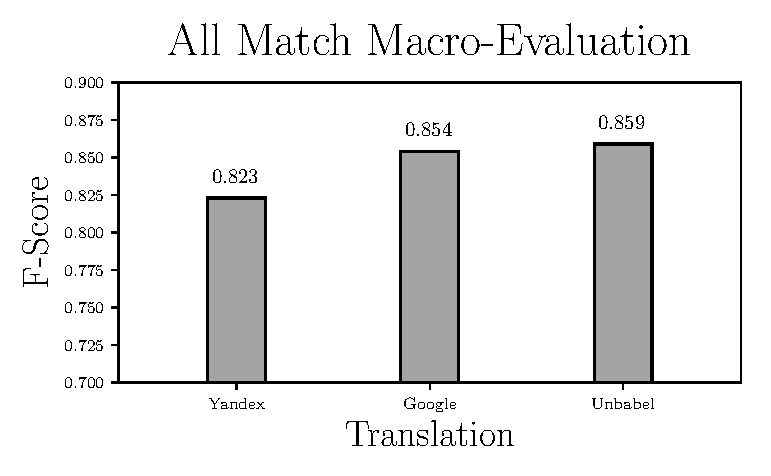
\includegraphics{SupportFiles/plots/All_Match_Macro_plot.pdf}


\section{Discussion}





\section{Conclusions}




  
